\clearpage

\section{Application to uncertainty propagation} \label{sec:aerospace_uncertainty}

After establishing the geometric features of transport maps on synthetic domains, the analysis focuses on the primary aerospace application: tracking uncertainty in orbital dynamics. The propagation of orbital vectors over time results in nonlinear deformations of the associated probability density. Accurately capturing these structural changes is essential for robust space situational awareness and orbit determination. The subsequent analysis employs the inexact optimal transport framework to approximate the mappings arising from physical orbital perturbations.

\subsection{Parameterisation of orbital state} \label{subsec:orbital_state}

The physical state of a satellite in orbit is conventionally defined by a set of parameters. A \emph{minimal set} establishes the smallest number of parameters required to fully identify the state of an object in orbit. For planar two-body orbits, the state information is contained in the satellite's position and velocity vectors, both three-dimensional. Thus, a minimal set of parameters will contain six entries. These orbits, also known as the Keplerian orbits, can take the form of two-dimensional conic sections: either circles, ellipses, parabolas, or hyperbolas. In classical celestial mechanics, the state is parameterised using the Keplerian orbital elements, which provide an intuitive geometric description of the trajectory. These six elements are defined as follows, and are visualised in Figure~\ref{fig:keplerian_elements} for a Low-Earth orbit satellite:
\begin{itemize}
    \item $a$: Semi-major axis, defining the spatial dimension of the orbital ellipse.
    \item $e$: Eccentricity, describing the deviation of the orbit from a circular trajectory.
    \item $i$: Inclination, representing the vertical tilt of the orbital plane relative to a referential plane.
    \item $\Omega$: Right ascension of the ascending node, specifying the horizontal orientation of the ascending intersection with the reference plane.
    \item $\omega$: Argument of periapsis, defining the orientation of the orbit within the orbital plane, relative to the point of closest approach to the main body.
    \item $\theta$: True anomaly, representing the angular position of the satellite along its trajectory at a specific epoch.
\end{itemize}

\begin{figure}[htbp]
    \centering
    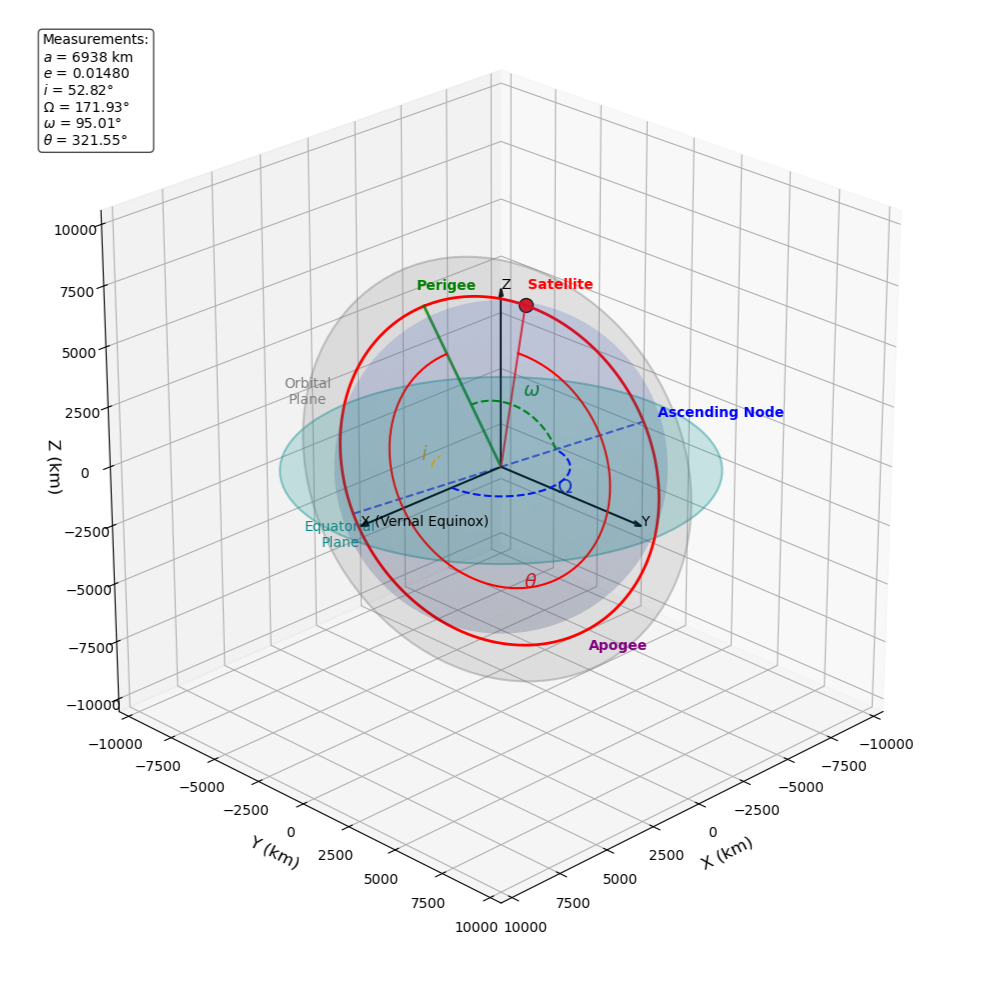
\includegraphics[width=\linewidth]{figures/Orbital_Plots_left.png}
    \caption{Geometric representation of the classical Keplerian orbital elements.}
    \label{fig:keplerian_elements}
\end{figure}
Additionally, the mean anomaly, $M$, is a mathematically convenient parameter that increases uniformly with time and represents the fraction of the orbital period elapsed since the satellite last passed periapsis. Although Keplerian elements provide geometric clarity, they exhibit mathematical singularities under specific conditions. For circular orbits ($e \to 0$), the argument of periapsis $\omega$ becomes undefined. For equatorial orbits ($i \to 0$ or $i \to 180^\circ$), the right ascension of the ascending node $\Omega$ is similarly undefined. These singularities introduce numerical instabilities during nonlinear state propagation and density-tracking procedures.

To address these computational limitations, it is standard practice to parameterise the state in terms of \emph{equinoctial elements}. This alternate formulation transforms the classical variables into a representation that remains nonsingular for circular and nonretrograde equatorial orbits. The equinoctial elements map the orbital state to a space defined by $\mathbb{R}^5 \times \mathbb{S}^1$, taking the following form:
\begin{itemize}
    \item $a$: Semi-major axis, retained from the classical formulation.
    \item $h$: First component of the eccentricity vector, evaluated as $h =e \sin(\omega + \Omega)$.
    \item $k$: Second component of the eccentricity vector, evaluated as $k =e \cos(\omega + \Omega)$.
    \item $p$: First component of the ascending node vector, evaluated as $p =\tan(i/2) \sin(\Omega)$.
    \item $q$: Second component of the ascending node vector, evaluated as $q =\tan(i/2) \cos(\Omega)$.
    \item $\lambda$: Mean longitude, incorporating the mean anomaly as $\lambda = \Omega + \omega + M$.
\end{itemize}

Tracking the probability distribution of the satellite state in equinoctial element space reduces the risk of algorithmic failure caused by coordinate singularities. In our framework, this parameterisation preserves the structural integrity of the optimal transport map during continuous integration of the physical dynamics. 

\subsection{Filtering} \label{subsec:filtering}

In space situational awareness, maintaining a robust representation of satellite uncertainty requires continuous evaluation of a probability density function under physical dynamics. Although transforming the state space into equinoctial elements mitigates the numerical singularities associated with classical orbital elements, the underlying orbital dynamics and measurement models remain fundamentally nonlinear. Therefore, sequential orbit determination requires \emph{filtering} techniques that can accommodate these nonlinearities. In the context of sequential orbit determination, filtering is defined as the recursive mathematical procedure for estimating the true physical state and its associated probability density, which operates by continually fusing noisy observational measurements with a predictive propagation model.

The standard approach in the aerospace literature is the Extended Kalman Filter (EKF), which operates by linearising the system dynamics and measurement models about the current state estimate~\cite{Horwood2014}. Although computationally efficient, this method assumes that the probability density function of the state uncertainty remains Gaussian throughout propagation. For typical orbital regimes, over extended propagation intervals, the distribution of uncertainty distributions undergoes nonlinear shearing, as visualised in Figure~\ref{fig:horwood_distributions}~\cite{Horwood2014}. Consequently, the EKF's uncertainty estimate will be structurally inappropriate for modelling the true probability distribution; at the same time, the filter may become ``overconfident'' in its estimate, resulting in degraded estimate accuracy and filter divergence.

To avoid explicit Jacobian calculations and reduce linearisation errors, the Unscented Kalman Filter (UKF) is often employed as an alternative to the EKF~\cite{Horwood2014}. Rather than directly linearising the equations, this filter deterministically propagates a minimal set of sample points through the true nonlinear functions to estimate the posterior mean and covariance~\cite{Horwood2014}. However, similarly to the EKF, the UKF assumes a Gaussian distribution. Thus, this filter also fails to represent the ground-truth probability distribution of the state, often assigning the highest probability mass to regions unoccupied by the satellite. This discrepancy results in a loss of realism in uncertainty representation.

When the Gaussian assumption is relaxed, Particle Filters (PF) provide a fully non-parametric alternative. By representing the uncertainty distribution as an ensemble of discrete, weighted Monte Carlo samples, PF methods can approximate arbitrary non-Gaussian geometries. However, standard particle filtering is susceptible to weight degeneracy, particularly in high-dimensional spaces or with sparse measurements, where a single particle accumulates most of the statistical weight, and the remainder are discarded. Advanced control-based techniques, such as the Nudged PF and its variational variants, have been developed to address sparse observations more robustly~\cite{Karampela2026}. Nonetheless, these sophisticated particle-based methods can often impose a computational burden that is prohibitive for real-time space situational awareness.

\subsection{Mapping Gauss von Mises distributions} \label{subsec:mapping_gauss_von_mises}

To combine the efficiency of analytical methods with the ability to represent the stretching topology of orbital uncertainty, we propose a hybrid approach that augments a Kalman filter with an optimal transport map. In particular, in this section, we demonstrate the effectiveness of the established inexact projection framework for mapping high-fidelity probability distributions to standard normals. We focus our attention on one such family of distributions, the Gauss von Mises (GVM) family~\cite{Horwood2014}. Defined on a cylindrical manifold, this distribution accommodates the nonlinear shearing inherent in long-term orbital propagations, thereby maintaining uncertainty realism over extended prediction horizons. Augmented with our optimal transport-derived deterministic transformation, the Kalman filter can perform its highly efficient measurement update on a theoretically Gaussian state, thereby integrating the high-fidelity orbital mechanics model into a computationally tractable architecture.

The formulation of the GVM distribution arises from the necessity to model uncertainties on the cylindrical manifold $\mathbb{R}^{D-1} \times \mathbb{S}^1$, where, as usual, $D$ represents the full state dimension. As discussed in Section~\ref{subsec:orbital_state}, for orbital element sets parameterising the state of a satellite in orbit, we adopt the equinoctial minimal set, and we thus have $D=6$. Partitioning the full state vector as $(v^T, \lambda)^T$, where $v \in \mathbb{R}^{5}$ denotes the linear coordinates (the first five equinoctial elements as defined in~\ref{subsec:orbital_state}), and $\lambda \in \mathbb{S}^1$ represents the bounded periodic angular coordinate (mean longitude). The probability density function of the GVM distribution is defined by coupling a multivariate Gaussian with a von Mises distribution~\cite{Horwood2014}. The joint probability density function is expressed as

\begin{equation} \label{eq:gvm_density}
\begin{aligned}
    p(v, \lambda) = \frac{1}{Z} \exp\Biggl( &-\frac{1}{2} (v - \mu_v)^T \Sigma_{vv}^{-1} (v - \mu_v) \\ 
    &- 2\kappa \sin^2\frac{1}{2}\big[\lambda - \mu_\lambda - \frac{1}{2}(L^{-1}(v - \mu_v))^T\Gamma (L^{-1}(v - \mu_v))\big] \Biggr),
\end{aligned}
\end{equation}
where $\mu_v$ and $\Sigma_{vv}$ are the mean and covariance of the linear coordinate subset $v$, $L$ is the lower-triangular Cholesky factor of $\Sigma_{vv}$ such that $\Sigma_{vv} = LL^T$,  $\mu_\lambda$ is the mean of the angular component $\lambda$, $\kappa$ is the concentration parameter defining the angular dispersion, and $\Gamma$ governs the structural correlation between the linear and periodic coordinates~\cite{Horwood2014}. The term $Z$ ensures the probability mass integrates to unity over the manifold. As the set of orbital elements is propagated through time, the nonlinear shear is accurately captured by the structural parameters $\Gamma$ and $\kappa$, allowing the probability contours to bend within the periodic domain without violating the topological boundaries.

\subsection{Numerical results} \label{subsec:gvm_numerical_results}

To assess the capability of the optimal transport framework to invert these orbital uncertainty distributions onto an isotropic domain, we conducted three separate numerical experiments. The common experimental pipeline employs a data generation module that instantiates the $n$ unmapped particles $\{x^{(i)}\}_{i=1}^n$ according to the GVM distribution in~\eqref {eq:gvm_density}. For each experiment, we specify a highly correlated covariance structure $\Sigma_{vv}$, a low concentration $\kappa$, and a dominant correlation vector $\Gamma$, to produce discrete state particles exhibiting the nonlinear crescent geometry characteristic of long-term orbital uncertainty propagation. The first experiment, which we denote as (a), aims to mirror the state of the satellite described in~\cite{Horwood2014} after propagation over 8 orbital epochs (see the bottom-right panel in Figure~\ref{fig:horwood_distributions}). The second experiment, denoted as (b), tests an even more extreme shearing case to simulate the effects of long-term propagation of orbital elements. The third experiment, denoted (c), evaluates the framework's robustness under a discontinuous, artificially truncated state distribution. This test was set up by generating the data according to the distribution in~\eqref {eq:gvm_density}, then filtering it according to a hard threshold constraint $\lambda \leq \bar{\lambda}$. In so doing, some particles were removed from the distribution altogether, rendering the optimiser's task to identify the map components $S^k$ significantly harder.

\begin{table}[htbp]
    \centering
    \caption{Distribution parameters for the orbital uncertainty experiments.}
    \begin{tabular}{lcccc}
        \toprule
        \textbf{Parameter} & \textbf{Symbol} & \textbf{(a)} & \textbf{(b)} & \textbf{(c)} \\
        \midrule
        Angular concentration & $\kappa$            & $5.2$ & $7.0$ & $5.2$ \\
        Correlation coefficient & $\Gamma_{11}$     & $2.4$ & $9.0$ & $2.4$ \\
        \bottomrule
    \end{tabular}
    \label{tab:orbital_gvm_parameters}
\end{table}

These three sets of generated particles constitute the source distribution for the mapping experiment. For a baseline Low-Earth orbit scenario, the initial state mean is initialised as $\mu_v = (\SI{7136.635}{\kilo\metre}, {0}_4)^T$ and $\mu_\lambda = 0$, where ${0}_4$ denotes a four-dimensional zero vector. The linear covariance matrix is set to $\Sigma_{vv} = \mathrm{diag}((\SI{20}{\kilo\metre})^2, 10^{-6}{1}_4)$ for all experiments, where ${1}_4$ represents the $4 \times 1$ vector of ones. Since the shearing effect is most prominent between the semi-major axis $a$ and mean longitude $\lambda$ elements in practical experiments, the correlation matrix is set to $\Gamma = \mathrm{diag}(\Gamma_{11}, 10^{-1}{1}_4)$, where $\Gamma_{11}$ dictates the specific magnitude of the along-track shear. These parameters are summarised in Table~\ref{tab:orbital_gvm_parameters}.

The remainder of the numerical setup is identical to that of previous experiments in this chapter. Simulation parameters for the three experiments are summarised in Table~\ref{tab:orbital_optimisation_parameters}.

\begin{table}[htbp]
    \centering
    \caption{Parameters for the orbital uncertainty experiments.}
    \begin{tabular}{lcccc}
        \toprule
        \textbf{Parameter} & \textbf{Symbol} & \textbf{(a)} & \textbf{(b)} & \textbf{(c)} \\
        \midrule
        Random seed & --                            & 8989 & 1234 & 1234567 \\
        State dimension & $D$                       & 6 & 6 & 6 \\
        Hermite degree & $J_k + 1$                  & 2 & 2 & 2 \\
        Particle count & $n$                        & 1000 & 2500 & 1000 \\
        Mini-batch cardinality & $B$                & 100 & 700 & 100 \\
        Outer PGD iterations & $T$                  & 1000 & 17,500 & 1000 \\
        Dykstra budget & $M_{\mathrm{base}}$        & 100 & 100 & 100 \\
        Budget scaling exponent & $p$               & 0.67 & 0.67 & 0.67 \\
        Initial learning rate & $\eta^\circ$        & 0.07 & 0.07 & 0.07 \\
        Learning rate decay & $\gamma$              & 0.01 & 0.01 & 0.01 \\
        IHT interval & $K_{\mathrm{IHT}}$           & 100 & 100 & 100 \\
        IHT tolerance & $\varepsilon_p$             & 0.01 & 0.01 & 0.01 \\
        Monotonicity tolerance & $\varepsilon_m$    & 1e-12 & 1e-12 & 1e-12 \\
        \bottomrule
    \end{tabular}
    \label{tab:orbital_optimisation_parameters}
\end{table}

To prevent the degeneration of the polynomial coefficients during optimisation, the empirical particle sets are preconditioned using a whitening procedure before training. Both the source and target distributions are initially transformed into a standardised space with zero mean and identity covariance. This affine projection eliminates severe structural correlations and scale disparities, resulting in a well-conditioned numerical environment in which Hermite basis functions can efficiently construct the transport map. In the whitened space, for the third experiment, we set the constraint value at $\bar{\lambda} = 5.0$, and matrix $L$ is obtained through standard Cholesky decomposition. After optimising the map within this standardised domain, the transported particles are projected back into the original physical coordinates by inverting the affine transformation using the target distribution's original scaling and shifting parameters.

Results for the three experiments are visualised in Figure~\ref{fig:gvm_combined_experiments}. The figure visualises a two-dimensional slice along the semi-major axis--mean longitude ($a$--$\lambda$) plane. The figure shows whitened values for ease of visualisation, since the large scaling of the dominant orbital element $a$ renders the plots otherwise illegible.

\begin{figure}[htpb]
    \centering
    \begin{subfigure}[b]{\linewidth}
        \centering
        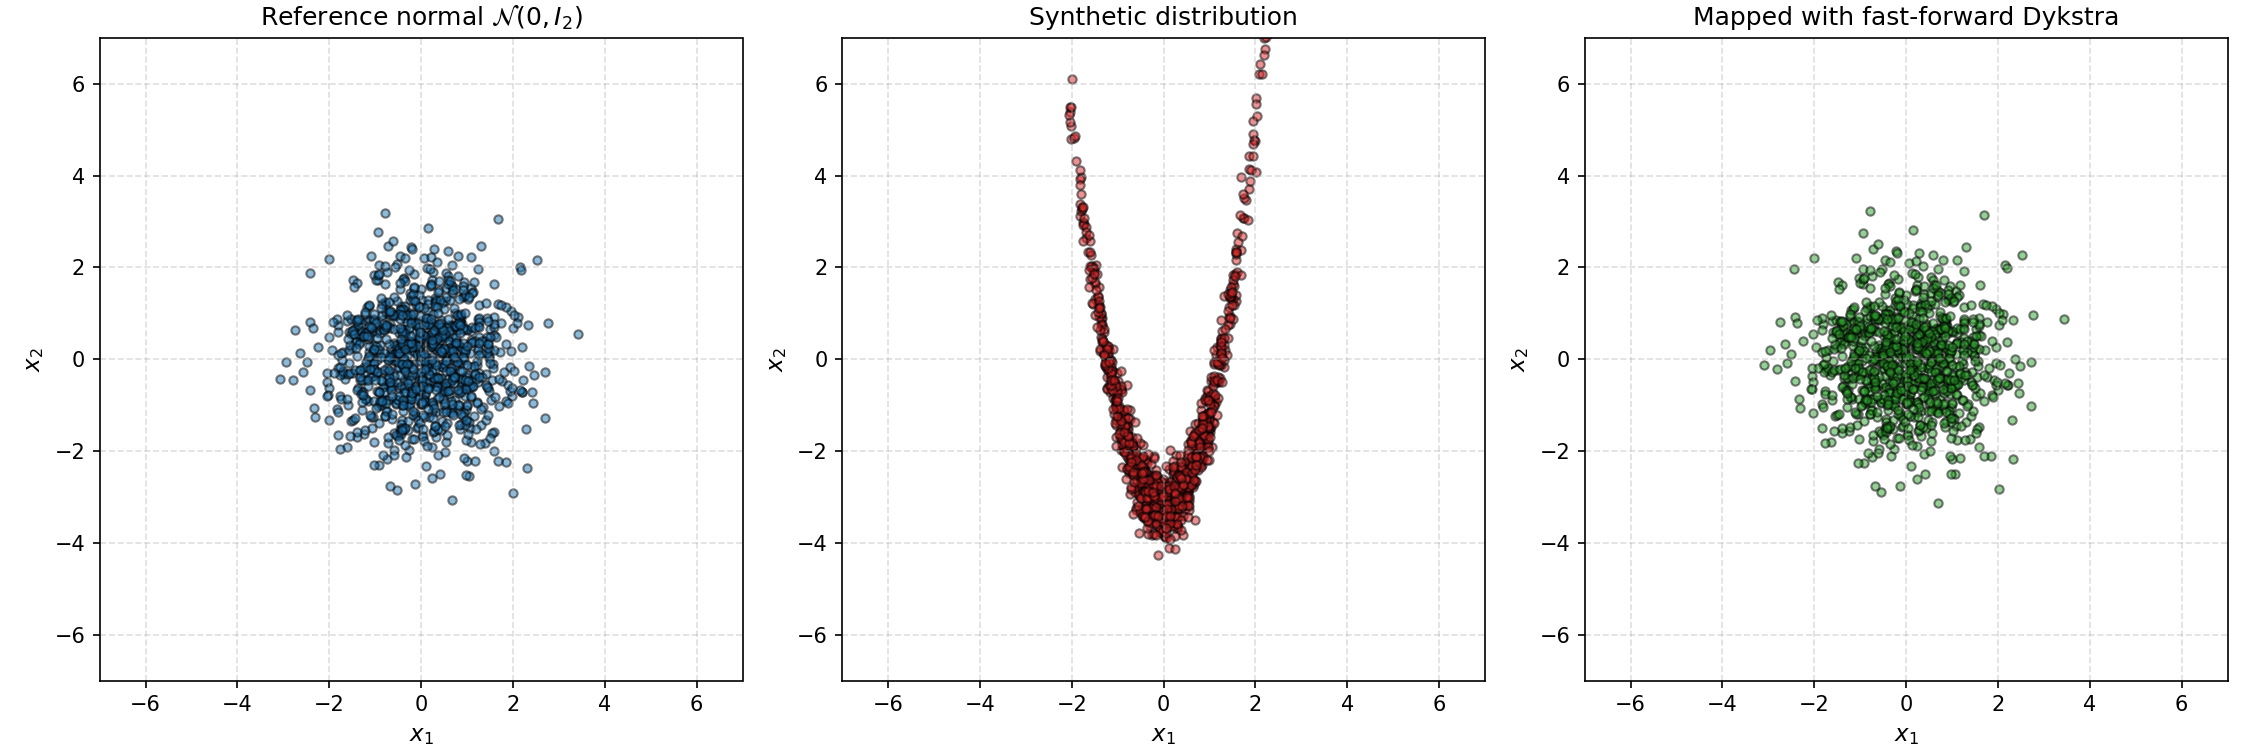
\includegraphics[width=\linewidth]{figures/kr2d_distribution_fast_SEED=8989_M=1000_D=2_SGD=100_PGDITERS=1,000_DYKSTRA_ITERS=1_10_L1=0.0_LR=7e-02_1e-02_IHT=100.png}
        \caption{Results for the baseline orbital propagation experiment (\texttt{SEED} $=8989$).}
        \label{fig:gvm_shear_a}
    \end{subfigure}
    
    \vspace{1em}
    
    \begin{subfigure}[b]{\linewidth}
        \centering
        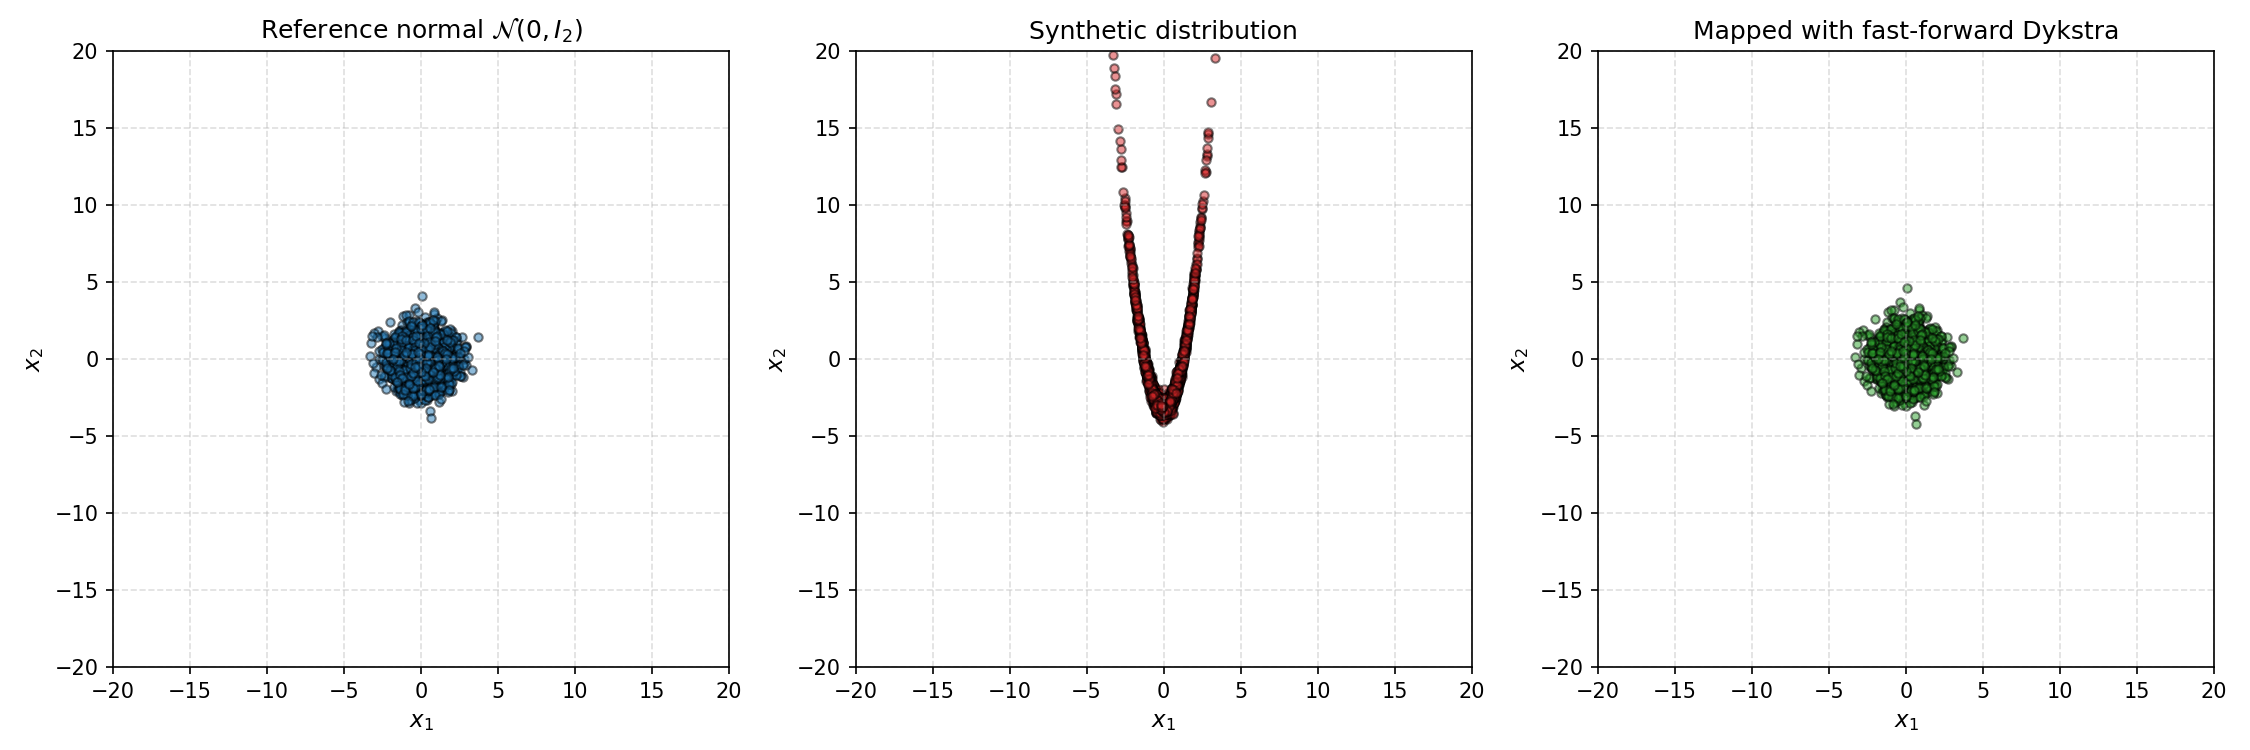
\includegraphics[width=\linewidth]{figures/kr2d_distribution_fast_SEED=1234_M=2500_SGD=700_PGDITERS=17,500_DYKSTRA_ITERS=1_10_L1=0.0_LR=7e-02_1e-02_IHT=100.png}
        \caption{Results for the extreme long-term orbital propagation experiment (\texttt{SEED} $=1234$).}
        \label{fig:gvm_shear_b}
    \end{subfigure}
    
    \vspace{1em}
    
    \begin{subfigure}[b]{\linewidth}
        \centering
        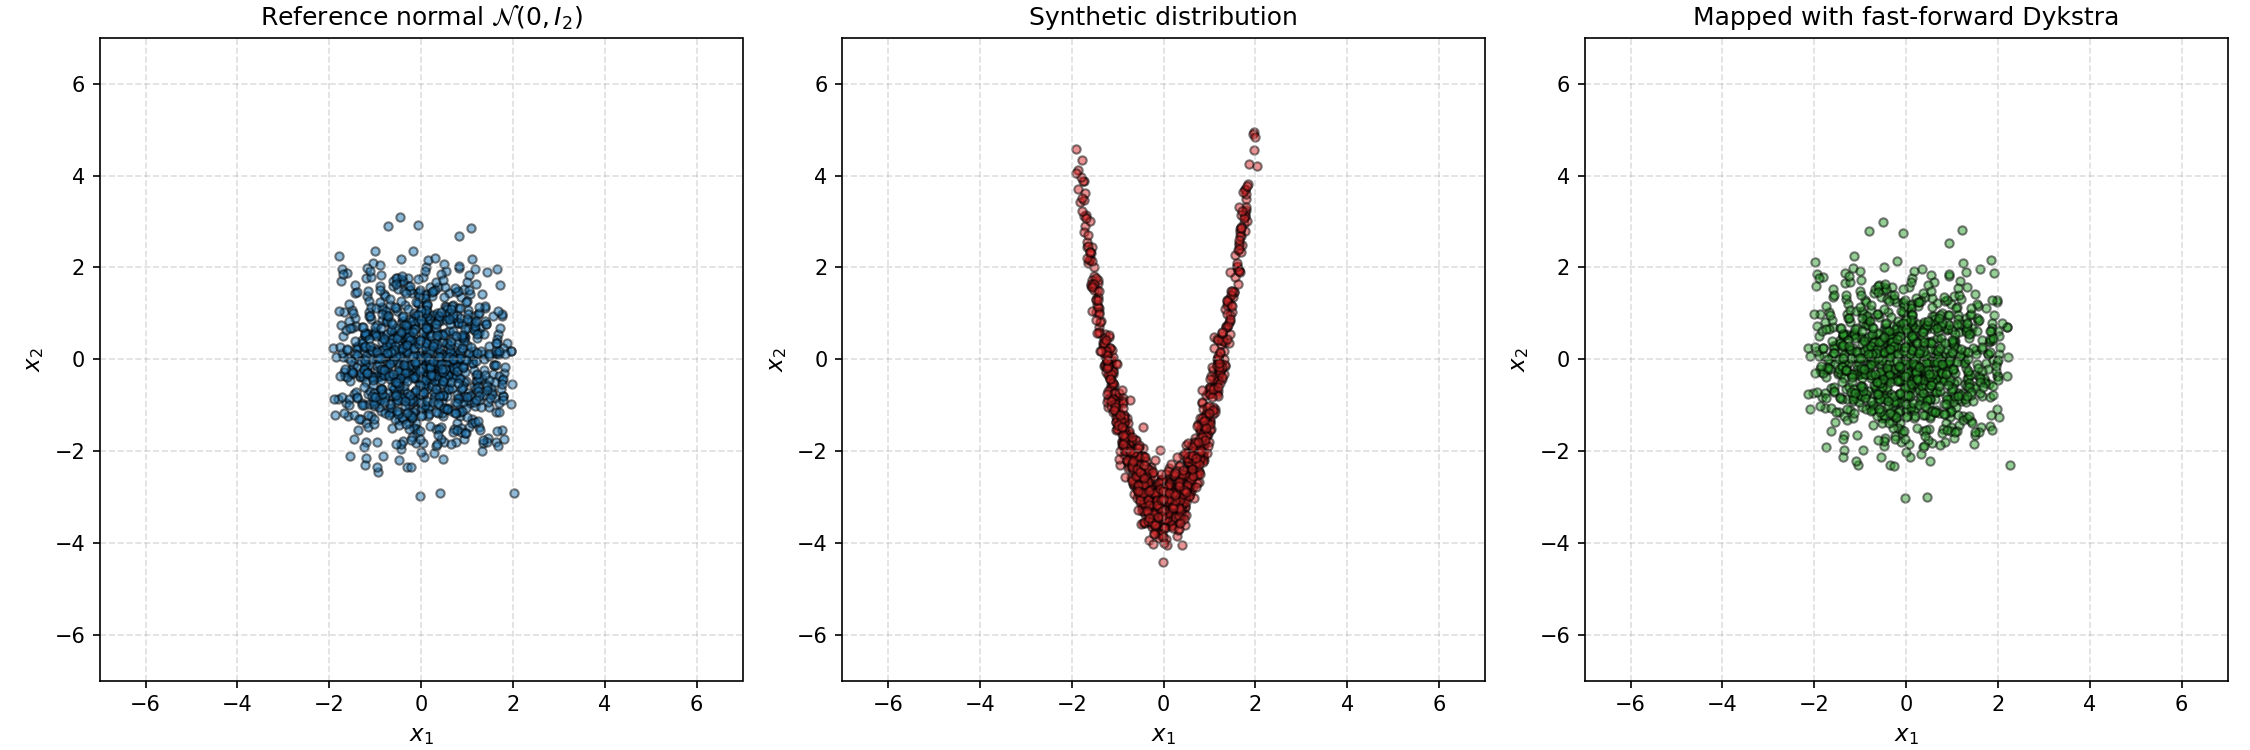
\includegraphics[width=\linewidth]{figures/kr2d_distribution_fast_SEED=1234567_M=1000_D=2_SGD=100_PGDITERS=1,000_DYKSTRA_ITERS=1_10_L1=0.0_LR=7e-02_1e-02_IHT=100.png}
        \caption{Results for the discontinuous orbital distribution experiment (\texttt{SEED} $=1234567$).}
        \label{fig:gvm_shear_c}
    \end{subfigure}
    
    \caption{Results for the three GVM orbital uncertainty experiments.}
    \label{fig:gvm_combined_experiments}
\end{figure}

Figure~\ref{fig:gvm_combined_experiments} confirms that the GVM distributions are successfully remapped to normal distributions. The empirical Wasserstein-2 distance between the mapped and unmapped distributions was consistently evaluated to be below $10^{-2}$ across all three configurations.

Static progress plots detailing the step-by-step structural deformation, which were provided for the lower-dimensional synthetic models, are omitted here for readability. Instead, complete temporal visualisations tracking the iterative convergence of the probability contours across all outer projected gradient descent loops have been rendered as animation videos. These are available for review, alongside those of synthetic and other runs, in the following shared folder:
\begin{center}
    \href{https://drive.google.com/drive/folders/1FEkJWo6-cSvWa-dAoq2DXf_d0Pf9xZye?usp=sharing}{https://drive.google.com/drive/folders/animation\_videos}
\end{center}

Table~\ref{tab:gvm_runtimes} details the empirical execution times required to optimise each independent scalar map component, $S^1$ through $S^6$, alongside the cumulative runtime, for the three experiments.

\begin{table}[htbp]
    \centering
    \caption{Computational runtime for the orbital uncertainty experiments.}
    \label{tab:gvm_runtimes}
    \begin{tabular}{@{}lcccccccc@{}}
        & & \multicolumn{7}{c}{Runtime (s)} \\
        \cmidrule(l){3-9}
        Experiment & Seed & $S^1$ & $S^2$ & $S^3$ & $S^4$ & $S^5$ & $S^6$ & Total \\
        \midrule
        (a) & 8989 & 8.0 & 22.6 & 36.6 & 49.1 & 61.0 & 81.0 & 258.3 \\
        (b) & 1234 & 296.4 & 853.4 & 1440.2 & 1779.5 & 2374.7 & 3029.9 & 9774.1 \\
        (c) & 1234567 & 11.8 & 32.4 & 54.1 & 74.4 & 92.0 & 116.6 & 381.3 \\
        \bottomrule
    \end{tabular}
\end{table}

As in previous runs, the component-level runtimes exhibit a monotonic scaling with increasing component dimension. This scaling reflects the growth of the Hermite polynomial basis necessary to parameterise the higher-dimensional conditional maps within the KR architecture. The severity of the initial nonlinear deformation directly influences the total algorithmic runtime. The baseline orbital scenario (a) and the artificially truncated state distribution (c) converged in 258.3 seconds and 381.3 seconds, respectively. Since these were stemming from the same distribution, with the only difference being the truncation constraint, we can conclude the optimiser found it harder to optimise the discontinuous distribution. By contrast, the extreme shear in scenario (b) required significantly greater computational effort, resulting in a cumulative runtime of 9774.1 seconds. Reversing stronger shears necessitates more outer stochastic gradient iterations to push the decision variables to higher overall values. We note that this example was deliberately made extreme, and that such vigorous distribution shears would only be encountered in very long-term propagations. Since Kalman filters are typically run sequentially at high frequency, this scenario is unlikely to arise in practice.

Despite the increased computational demands associated with the most extreme propagation horizons, these results collectively confirm the robustness of the inexact projection solver when applied to high-fidelity, dimensionally complex aerospace distributions. By reliably enforcing monotonicity and recovering the standard normal geometry from highly sheared equinoctial states, this optimal transport framework demonstrates its suitability as a deterministic transformation mechanism for augmenting the standard Kalman filter architecture.